%!TEX root = ../artigo.tex
\section{sintelo} % (fold)
\label{sec:sintelo}
A ferramenta sintelo é uma ferramenta didática para o ensino de compiladores. A mesma foi criada por Karina Kieling Dos Santos e Philipe Marcon Dos Reis, no ano de 2008 como Trabalho de Conclusão de Curso pela Universidade
do Sul de Santa Catarina e foi publicada em \cite{sintelo}. 

Embora a ferramenta em questão possua mais funcionalidades, esse trabalho se limitou a parte de análise léxica, permanecendo em seu escopo.

Para que possamos realizar a análise léxica, primeiramente devemos informar ao sintelo os tokens de nossa linguagem, através de expressões regulares. Essas expressões regulares devem ser informadas na ``caixa'' chamada léxico, conforme ilustrado na figura~\ref{sintelo-inicial}.

\begin{figure}[ht!]
	\centering
	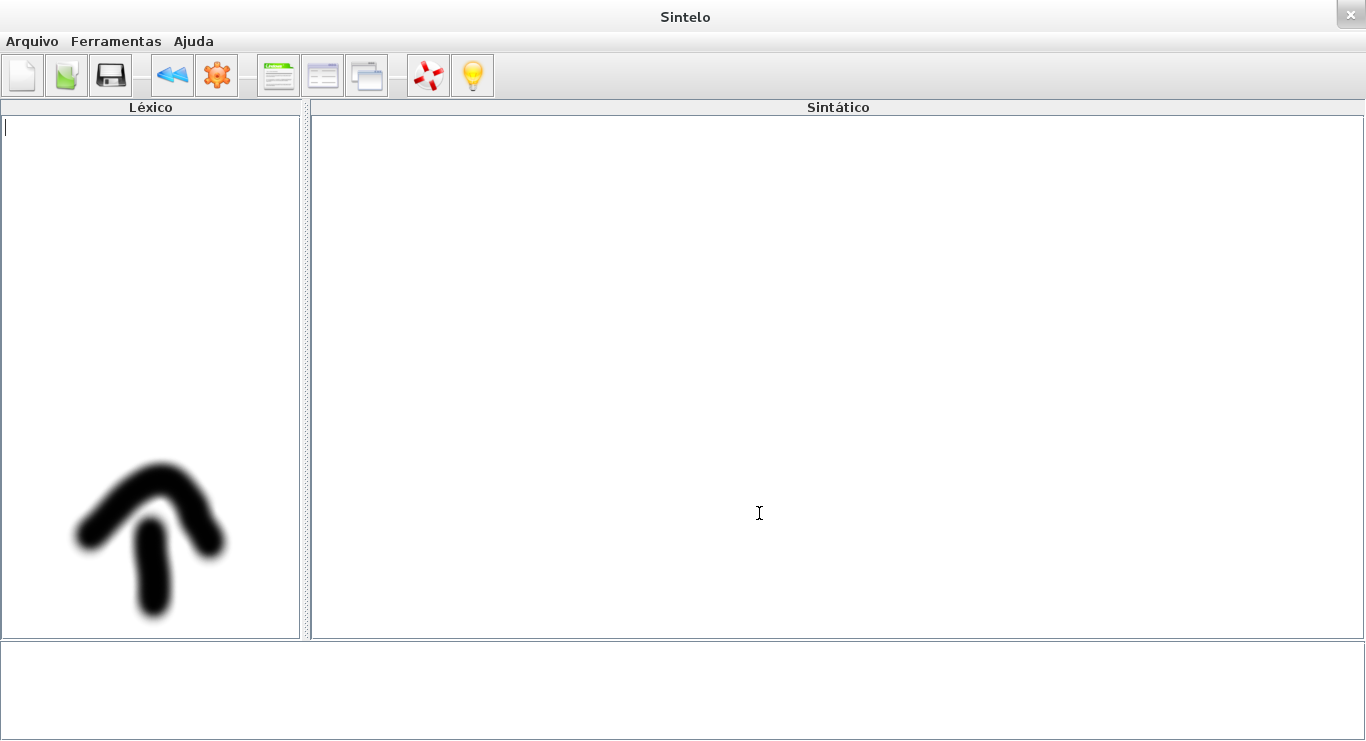
\includegraphics[scale=0.28]{imgs/sintelo-inicial-ed}
	\caption{Tela inicial do sintelo}
	\label{sintelo-inicial}
\end{figure}

A notação utilizada para representar as expressões regulares são descritas em \cite{sintelo} ou no manual da ferramenta, que pode ser acessado através do menu ``Ajuda'', item ``Manual'' e seção ``Especificações Léxicas''. Desta forma este artigo não explicará a notação.

Para exibir a análise léxica, o exemplo de operações aritméticas de \cite{Sebesta201201} será adaptado. Esse exemplo reconhece operações aritméticas que podem conter números (inteiros e/ou reias), identificadores (variáveis), operações binárias e também parêntesis; ignorando espaços em branco, quebra de linha e tabulação.

A seguir, a especificação dos tokens que deve ser passada para o sintelo:
\begin{verbatim}
ID:[a-zA-Z_][_a-zA-Z0-9]*
INT:[0-9]+
REAL:([0-9]\.[0-9]+) | ([0-9]+\.[0-9])
"("
")"
binop:"+" | \- | \*|"/"
:[\s\n\t]+
\end{verbatim}


% section sintelo (end)